Topos theory arose in the 1960s as a geometric concept in the work of Grothendieck and others in algebraic geometry. They defined a topos as a category equivalent to the category of sheaves $\sh(C,J)$ on some site $(C,J)$. Sites axiomatize and generalize the notion of open covering from topology, where the objects of $C$ are the generalized open sets and $J$ is a Grothendieck topology, which will be defined later. Suffice it to say that for each topological space $X$, the poset of open subsets of $X$ considered as a category gives rise to a site. Grothendieck toposes a special case of the more general notion of elementary toposes, which were introduced by Lawvere and Tierney. While Grothendieck's school sought to construct a general framework for doing geometry in an effort to construct a suitable cohomology theory for schemes, Lawvere and Tierney emphasize the role of the subobject classifiers for working in the internal logic of a topos. The subobject classifier $\Omega$ for some (elementary) topos $\mathcal{E}$ is a generisation of the following situation:
For a subset $S \subset X$, there is a characteristic function $\char \colon X \to \{0, 1\}$ of $S$ given by
\[ \char_S(x) =
	\begin{cases}
		\ 1,\ x \in S, \\
		\ 0,\ x \not \in S,
	\end{cases}
\]
where $0$ is interpreted as the truth value \textbf{false} and $1$ is interpreted as \textbf{true}. Each subset $S$ of $X$ can be recovered by its characteristic function by pulling back \textbf{true} along $\char_s$. This means that the subobject functor $\text{sub} \colon \Set \to Set$ which sends a set $S$  to its powerset $\mathcal{P}(S)$ is representable.

\begin{construction}[Subobjects]
	Recall that a morphism $f \colon A \to B$ in any category is called a monomorphism if for any object $C$ and parallel arrows $g, h \colon C \xbigtoto{} A$ with $fg = fh$ implies $g = h$. We consider two monomorphisms $f \colon A \to B$ and $f' \colon A' \to B$ to be equivalent if there is an isomophism $A \simeq A'$ with $f'h = f$
\end{construction}

Every Grothendieck topos posesses such an a subobject classifier $\Omega$. This object allows us to construct subobjects $\{x \mid \varphi(x)\} \subset X$ for each object $X$ of $\mathcal{E}$ in much the same way as in the category of sets by using a language $\mathcal{L}$ constructed from the objects of the topos $\mathcal{E}$. This language has a nice semantic interpretation in the case of Grothendieck toposes $\sh(C,J)$. There is the \textit{forcing relation} $\Vdash$ which is defined for an object $U \to X$ over $X$ in the over-category $C/X$ and $\varphi(x)$ is a term in a suitable type theory with a free variable of type $X$. We define $U \Vdash \varphi(x)$ to hold if $U \to X$ factors through a map $U \to \{x \mid \varphi(x)\}$ as indicated in the diagram below:
\[
	% https://q.uiver.app/?q=WzAsNSxbMCwxLCJVIl0sWzEsMSwiWCJdLFsxLDAsIlxce3ggXFxtaWQgXFx2YXJwaGkoeClcXH0iXSxbMiwwLCJcXG1hdGhiZnsxfSJdLFsyLDEsIlxcT21lZ2EiXSxbMCwxXSxbMCwyLCIiLDIseyJzdHlsZSI6eyJib2R5Ijp7Im5hbWUiOiJkYXNoZWQifX19XSxbMiwzXSxbMyw0LCJcXHRleHR7dHJ1ZX0iLDJdLFsyLDFdLFsxLDRdXQ==
	\begin{tikzcd}
		& {\{x \mid \varphi(x)\}} & {\mathbf{1}} \\
		U & X & \Omega
		\arrow[from=2-1, to=2-2]
		\arrow[dashed, from=2-1, to=1-2]
		\arrow[from=1-2, to=1-3]
		\arrow["{\text{true}}"', from=1-3, to=2-3]
		\arrow[from=1-2, to=2-2]
		\arrow[from=2-2, to=2-3]
	\end{tikzcd}
\]
Here $\{ x \mid \varphi(x)\}$ is defined as the subobject arising from the map $\varphi(x) \colon X \to \Omega$. In chapter TODO we will see how this map arises when $\varphi(x)$ is a term of the internal language $\mathcal{L}$. If the dotted map exists, interpret this as saying that $\varphi(x)$ holds locally on $U$. This leads naturally to the notion of cohomology, which measures the obstruction from constructing global solutions from local solutions.\par

We will take an in depth look at a particular example: The \'etale topos of a scheme. We first develop the theory of \'etale maps and their Galois theory. This theory generalises classical Galois theory from fields to schemes and will allow us to define the fundamental group $\pi_1^{\et}(X)$ of a connected scheme $X$. Then we introduce the notion of site and define sheaves on sites, directly generalizing sheaves on topological spaces. We then take a closer look at sheaves on the \'etale site of a scheme and study their cohomology. We also give an introduction to the internal logic of the \'etale topos, which will allow us to speak of sentences being true locally on an \'etale open $U \to X$.\par

There are multiple good reasons to consider \'etale morphisms. One is that \'etale maps behave much like local homeomorphisms in topology and yield a good covering theory, which allows us to define fundamental groups of schemes. Another reason is that in a certain sense the \'etale topology is much finer that the Zariski topology, allowing us to trivialize bundles and coverings over \'etale open covers $\coprod U_i \to U$.\par

The absolute Galois group $\Gal(\Q) = \G_\Q$ of the rational numbers is one of the most important but also one of the most intractable objects in number theory. It is conjectured that every finite group arises as a subgroup of $\G_\Q$. In order to understand this large profinite group, we could study the representations of $\G_\Q$, which are homomorphisms $\G_\Q \to \GL_n(V)$, where $V$ is a finite dimensional $\Q$-vector space. It is not at all clear how to obtain such representations. Galois representations of $G_\Q$ arise from \'etale cohomology of varieties over $\Q$

\section{Prerequisites}
We assume aqcuaintance with the basics of category theory including limits and adjoint functors. This text contains a brief reminder of the Yoneda lemma. We will make free use of results from commutative algebra and field theory but will provide definitions and references wherever needed. We will also use basic notions of scheme theory and homological algebra.

\section{Conventions}
We denote the Yoneda embedding by $\yo \colon C \to \Set^{C^{op}} = \widehat{C}$


\section{Reminder on Schemes and the Zariski Topology}
The basic building blocks of algebraic geometry are affine schemes. An affine scheme $\Spec(A)$ is a geometric object constructed out of the prime spectrum
\[
	\Spec(A) = \{p \subseteq A \mid p \text{ prime ideal}\}
\]
of a commutative ring $A$. We would like to interpret the ring $A$ as the ring of functions on $\Spec(A)$, analogous to the ring
$\Sh{O}(M) := \{f: M \to \R \mid f \text{ continuous}\}$
for a manifold $M$. As a notational trick we write $f(p)$ for the image of $f$ under the quotient map $A \to A/p$. Note that the domain of a function $f$ depends on where it is evalued! The function $f \in A$ sends a point $p \in \Spec(A)$ to $f(p) = \overline{p} \in A/p$.  We will often consider schemes over a field, which are schemes equipped with a morphism $X \to \Spec(k)$, $k$ a field. This field will then play the role of $\R$ as in the example of manifolds. We equip $\Spec(A)$ with the Zariski topology, which has a basis given by sets of the form
\begin{align*}
	D_f & = \{ p \in \Spec(A) \mid (f) \not \subseteq p \} \\
	    & = \{ p \in \Spec(A) \mid f(p) \neq 0\}.
\end{align*}
\begin{definition}
	The \textit{Zariski topology} on $\Spec(A)$ consists of open sets of the form $D_I = \{ p \in \Spec(A) \mid I \not \subset (p)\}$ where $I \subseteq A$ is an ideal. The closed sets are of the form
	\begin{align*}
		V_I & = \{ p \in \Spec(A) \mid I \subseteq p \}              \\
		    & = \{ p \in \Spec(A) \mid f(p) = 0\ \forall f \in I \},
	\end{align*}
	the \textit{vanishing set} or \textit{zero locus} of $f$.
\end{definition}

Since $f(p) \neq 0$ for all $p \in D_f$, we view the ring $A[1/f]$ as the ring of rational functions defined on $D_f$. It consists of elements of the form
\[
	\biggl\{ \frac{g}{f^k} \mid g \in A, k \in \N \biggr\}.
\]
The assingment $D_f \to A[1/f]$ extends to a sheaf $\Sh{O}_{\Spec(A)}: \Spec(A) \to \mathsf{Ring}$, called the \textit{structure sheaf of $\Spec(A)$}. This sheaf has the property that the ring of global sections, denoted by $\Gamma(\Spec(A), \Sh(O)_{\Spec(A)}$ is isomorphic to $A$. We obtain a pair of functors
\begin{align*}
	\Spec :  \text{CRing}^{op} & \to \text{LRS} \\
	A                          & \to \Spec(A)
\end{align*}
from the category of commutative rings to the category of locally ringed spaces. An affine schemes is a locally ringed space isomorphic to $\Spec(R)$ for some ring $R$. A scheme is a locally ringed space with a covering by affine schemes. The functor seding an affine scheme $\Spec(A)$ to the ring of global sections of the structure sheaf $\Sh{O}_{\Spec(A)}$ is fully faithful and induces a bijection

\[
	\Hom_{\text{CRing}}(R, \Gamma(Y,\Sh{O}_Y)) \cong \Hom_{\text{Sch}}(Y, \Spec(R))
\]

Basic examples of affine schemes arise from polynomial rings: scheme-theoretically, the zero locus of a polynomial $f \in k[x_1, \dots, x_n]$ is given by the affine scheme $\Spec(k[x_1, \dots, x_n]/(f))$, for instance the parabola is $\Spec(k[x,y]/(x^2-y))$.

\begin{proposition}
	For a commutative ring $R$,
\end{proposition}

\begin{definition}
	A \textit{scheme} is a locally ringed space $X$ such that there is a covering $\{U_i\}_{i \in I}$ of $X$ such that each $U_i$ is isomorphic to an affine scheme $\Spec(A_i)$ for some ring $A_i$.
\end{definition}

Suppose $X = \Spec(A)$ is an affine scheme. If $\mathfrak{p} \subset \mathfrak{q}$ are two prime ideals of $A$, one contained in the other, then the neighborhood filter of $\mathfrak{p}$ is contained in the neighborhood filter of $\mathfrak{q}$. This induces a binary relation and in fact a partial order on the points of $X$. We say that $x$ \textit{is a specialization of} $y$ if $x \in \overline{y}$.

\begin{example}
	Let $A$ be a valuation ring of a field $K$, which means that for all $x \in K$ one has $x \in A$ of $x^{-1} \in A$. Then the ideals of $A$ are totally ordered by inclusion: We have a unique maximal ideal which consists of those $x \in K$ for which $v(x) \ge 0$, where , which corresponds to a uniqe closed point in $\Spec(A)$

	\begin{lemma}
		Let $R$ be a valuation ring of with fraction field $K$. The ideals of $R$ are totally ordered by inclusion.
	\end{lemma}

	\begin{proof}
		Let $I$ and $J$ be two ideals of $A$ with $I$ not contained in $J$, pick $a \in I \setminus J$. If $b \in J$, we must show that $b \in I$. If $b = 0$ we are done. Now let $b \neq 0$. We have $b/a \in R$, because otherwise $a/b$ in $R$ which would imply $a = (a/b)b \in J$, which is a contradiction. Therefore $b = (b/a)a \in I$.
	\end{proof}
\end{example}

We view elements of a ring $R$ as functions defined on $\Spec(R)$. If we have two subsets $A \subset B$ of $R$, then $V(B) \subset V(A)$, so $V(B)$ is a \textit{special subset of $V(A)$}, satisfying more conditions than $V(B)$.

\section{Motivation for Cohomology}
One of the most important invariants of schemes is \'etale cohomology.  Cohomology is an important invariant in geometry and topology which associates to each space $X$ a sequence of abelian groups $H^i(X)$, $i \ge 0$, the cohomology groups of $X$. For each map $f: X \to Y$ of spaces there are homomorphisms $f^*: H^i(Y) \to H^i(X)$. Moreover there are so called coboundary morphisms $\partial^i : H^i \to H^{i+1}$ for each $i \ge 0$.
\begin{definition}
	A \textit{cohomology theory} for
\end{definition}
We can deduce many interesting properties of spaces from their cohomology groups and the associated homomorphisms.

An important and intuitive cohomology is \textit{singular cohomology}. It provides a rigorous way for counting ``holes'' in a topological space. For instance, the circle $S^1$ has 1 one-dimensional hole while the torus $T^2$ has 2. The sphere $S^2$ has 1 two-dimensional hole but no one-dimensional holes, in symbols\footnote{$\Z$ appears here because it is the free group on one generator.}
\begin{align*}
	H^1_{sing}(S^1) \simeq \Z,\quad & H^1_{sing}(T^2) \simeq \Z \oplus \Z, \\
	H^1_{sing}(S^2) \simeq  0,\quad & H^2_{sing}(S^2) \simeq \Z.
\end{align*}
A general approach to cohomology is to use sheaves on a topological space as ``coefficients''. Sheaves consist of local data on a space that is glueable. A basic example consists of functions on a space: If we have an open cover $\{ U_i\}$ for a manifold $M$ and functions $f_i: M \to \R$ that agree on all intersections $U_i \cap U_j$ we may patch it together to a function $f: M \to \R$.
For any space $X$ and any sheaf $\Sh{F}$ on $X$ we can define $H^i(X, \Sh{F})$. Many examples of cohomology theories turn out to stem from the cohomology of a particular sheaf. For example, if $X$ is a locally contractible space, the singular cohomology $H_{\text{sing}}^i(X)$ of $X$ is isomorphic to the sheaf cohomology $H^i(X, \Z_X)$ of the constant sheaf $\Z_X$ on $X$.

One of the main motivations for \'etale cohomology is that one would like a replacment for singular cohomology for schemes. There are a number of obstacles:
\begin{proposition}\label{scheme_contractible}
	An irreducible scheme is contractible.
\end{proposition}
\begin{proof}
	Define a map $f: X \times I \to X$  by $f(x,0) = x$ and $f(x,t) = \eta$ for $t > 0$. This is a contraction of $X$ onto the point $\eta$, so the singular cohomology of $X$ is identically 0.
\end{proof}

\begin{proposition}
	$H^i(X, \Sh{F})$ is 0 for any sheaf on an irreducible topological space.
\end{proposition}
\begin{proof}
	See section TODO.
\end{proof}
This is a strong indication that the traditional tools of cohomology are inadequate to analyse the geometry of schemes.


\section{Fundamental groups}
Another important invariant of spaces is the fundamental group. The fundamental group of a pointed topological space $(X,x)$, denoted by $\pi_1(X,x)$ may be defined in two equivalent ways: Via homotopy classes of loops in $X$ based at $x$, or as the automorphism group of the fiber functor $F_x: Cov(X) \to Set$. From the first perspective, the fundamental group measures the connectivity of a space. The construction makes use of the unit interval. The unit interval $[0,1] \subset \R$ is not an algebraic set so the first definition does not have a natural formulation using only the notions of algebraic geometry. The second approach yields a theory strongly reminiscent of Galois theory. Grothendieck pioneered this approach in algebraic geometry.

\subsection{The fundamental group via paths}
A loop with base point $x$ is a map $\gamma : [0,1] \to X$ such that $\gamma(0) = \gamma(1) = x$. The homotopy class of $\gamma $ is denoted by $[\gamma]$. Define a composition operation by concatenation: $[\gamma] \circ [\eta] = [\gamma \circ \eta]$, where $\gamma \circ \eta$ is defined to be the path
\[
	\gamma \circ \eta =
	\begin{cases}
		\ \eta(2x) \text{ for } x \in [0, \tfrac{1}{2}] \\
		\ \gamma(2x - 1) \text{ for } x \in [\tfrac{1}{2}, 1].
	\end{cases}
\]
It is clear that this construction yields a group structure on the set
\[
	\{\ [\gamma] \mid \gamma : [0,1] \to X , \gamma(0) = \gamma(1) = x \}
\]
of homotopy classes of loops at $x$.

\subsection{The monodromy action}

\begin{construction}[Covering spaces]
	Let $X$ be a topological space. A \textit{space over $X$ } is a topological space $Y$ together with a continuous map $Y \to X$. A morphis between two spaces $Y_1, Y_2$ over $X$ is a continuous map $f: Y_1 \to Y_2$ such that the diagram
	\[
		% https://q.uiver.app/?q=WzAsMyxbMCwwLCJZXzEiXSxbMiwwLCJZXzEiXSxbMSwxLCJYIl0sWzAsMSwiZiJdLFsxLDIsInBfMiJdLFswLDIsInBfMSIsMl1d
		\begin{tikzcd}
			{Y_1} && {Y_1} \\
			& X
			\arrow["f", from=1-1, to=1-3]
			\arrow["{p_2}", from=1-3, to=2-2]
			\arrow["{p_1}"', from=1-1, to=2-2]
		\end{tikzcd}
	\]
	commutes. We obtain the category $\Top/X$ of spaces over $X$. A space $f: Y \to X$ over $X$ is called a local homeomorphism if for any point $y \in Y$ there is a neighborhood $U$ of $x$ such that the preimage $f^{-1}(U)$ is homeomorphic to a disjoint union of the open sets $f^{-1}(U) \cong \coprod U_i$ such that each $U_i$ gets mapped to $U$ homeomorphically under $f|_{U_i}$. Surjective local homeomorphisms over a space $X$ are also called \textit{covering spaces of $X$} or simply \textit{coverings}. Let $f: Y \to X$ be a surjective local homeomorphism. A trivial covering is one of the form $p: \coprod X \to X$, where $p$ restricts to the identity on each component. Using this terminology one can also say that a covering is a \textit{locally trivial local homemorphism}.
\end{construction}

\begin{lemma}[Path-lifting property of covering spaces]
	Let $p: Y \to X$ be a cover, $y \in Y$ and $x = p(y) \in X$.
	\begin{enumerate}
		\item If $f: [0,1] \to X$ is a path in $X$ with $f(0) = x$, then there is a unique path $\tilde{f}: [0,1] \to Y$ with $\tilde{f}(0) = y$ and $p \circ \tilde{f} = f$
		\item Assume we have a second path $g \colon [0,1] \to X$ homotopic to $f$ with the same endpoints. Then the unique lift $\tilde{g}$ of $g$ to $Y$ is homotopic to $\tilde{f}$ with the same endpoints.
	\end{enumerate}
\end{lemma}

\begin{proof}
	See \cite{Szamuely}, Lemma 2.3.2.
\end{proof}

\begin{construction}[The monodromy action]
	Let $p(y)=x$ and let $\alpha \in \pi_1(X,x)$ be represented by a path $f: [0,1] \to X$. By the previous lemma, there is a unique lift $\tilde{f}$ with $\tilde{f}(0) = y$. Since $p \circ \tilde{f} = f$, we have $(p \circ \tilde{f})(1) = x$, so the fundamental group $\pi_1(X, x)$ acts on $F_x(Y)$. This action is called the \textit{monodromy action}.
\end{construction}

A $Y$-automorphism is defined to be an automorphism of $Y$ in $\Top/X$. Let $Cov(X)$ be the subcategory of $\Top/X$ consisting of covering spaces. For each point $x \in X$ there is a functor $F_x: Cov(X) \to \Set$, sending a covering $p: Y \to X$ to the set $\{y \in Y \mid p(y) = x\}$. Now define an automorphism of $F_x$ to be a natural transformation $\psi: F_x \to F_x$ with a two-sided inverse. The set $\text{Aut}(F_x)$ of automorphisms of $F_x$ carries the structure of a group by composition. Note that for a covering $Y$ of $X$ and an automorphism $\phi \in \text{Aut}(F_x)$, there is by definition a morphism $\phi(Y): F_x(Y) \to F_x(Y)$. We define $\pi_1(X,x)$ to be the automorphism group of $F_x$.

We would like to have a notion of fundamental group for schemes. As before, there are some obstacles:

\begin{itemize}
	\item As we have seen in~\ref{scheme_contractible}, any irreducible scheme $X$ is contractible. As every loop in an irreducible scheme is contractible, this implies that $\pi_1(X)$ is $0$. In a sense this means that the unit interval is not a suitable ``test space'' to probe varieties and schemes.
	\item There is no universal covering space.
	      For instance, the algebra homomorphism given by $x^n \to x^n, k[x^n] \to k[x]$ corresponds to a map $x \to x^n, \mathbb{A}^1_k \to \mathbb{A}^1_k$. Depicted is the map from $\mathbb{A}^1_\C$ to $\mathbb{A}^1_\C$ for the case $n=2$

	      %  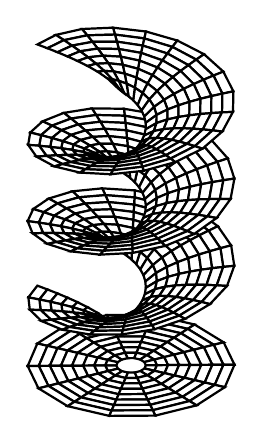
\begin{tikzpicture}[scale=2]
    \begin{axis}[
        axis lines=none,
        axis equal image,
        trig format plots=rad,
        z buffer=sort]
   \addplot3 [
        surf,
        domain=1:7,
        domain y=-pi:pi,
        samples=9,
        samples y=15,
        shader=flat,
        draw=black,
        fill=white
        ]
    ({x*cos(y)},{x*sin(y)},{-12});
   \addplot3 [
        surf,
        domain=1:7,
        samples=9,
        samples y=60,
        shader=flat,
        draw=black,
        fill=white,
        domain y=-3*pi:3*pi
        ]
    ({x*cos(y)},{x*sin(y)},{ln(x)+ y});
    \end{axis}
  \end{tikzpicture}




	      This map \textit{should} be local homeomorphism, but this is false in the Zariski topology. There do not exist nonempty open subsets $V$ and $U$ such that $x \to x^n$ maps $V$ isomorphically onto $U$. The theory of \'etale coverings will give us a good notion of covering which we will use to define the analog of universal coverings
\end{itemize}

The \'etale topology will provide a solution for the problems we have with both cohomology and fundamental groups. The \'etale topology is not a topology in the classical sense, but a category equipped with a notion of covering (in the sense of point-set topology). The analog of open sets of a scheme $X$ will be so called \'etale morphisms $U \to X$. \'Etale morphisms are the natural analogs of local homeomorphisms in scheme theory, so they provide a finer topology than the Zarisiki topology, giving rise to a better sheaf theory. Furthermore, surjective \'etale morphisms share a lot of formal properties with covering spaces, allowing us to define the \'etale fundamental group $\pi_1^{\et}$.
